\section{\acf{DTN}}

\subsection{Introduction}

\begin{frame}
  \frametitle{\acf{BP7}}

  \begin{itemize}
  \item Describes both a \acs{DTN} architecture and protocol
  \item Still in active development
  \item Latest draft was released on 04.08.2019
  \item Aims to obsolete Bundle Protocol Version 6, RFC 5050
  \end{itemize}
\end{frame}

\subsection{Nodes and Endpoints}

\begin{frame}
  \frametitle{Nodes and Endpoints}

  \begin{itemize}
  \item Nodes are identified by an Endpoint ID (URI), e.g., \texttt{dtn:node}
  \item A node might be addressed by multiple Endpoint IDs
  \item An Endpoint ID might represent multiple nodes
  \end{itemize}

  \begin{figure}
    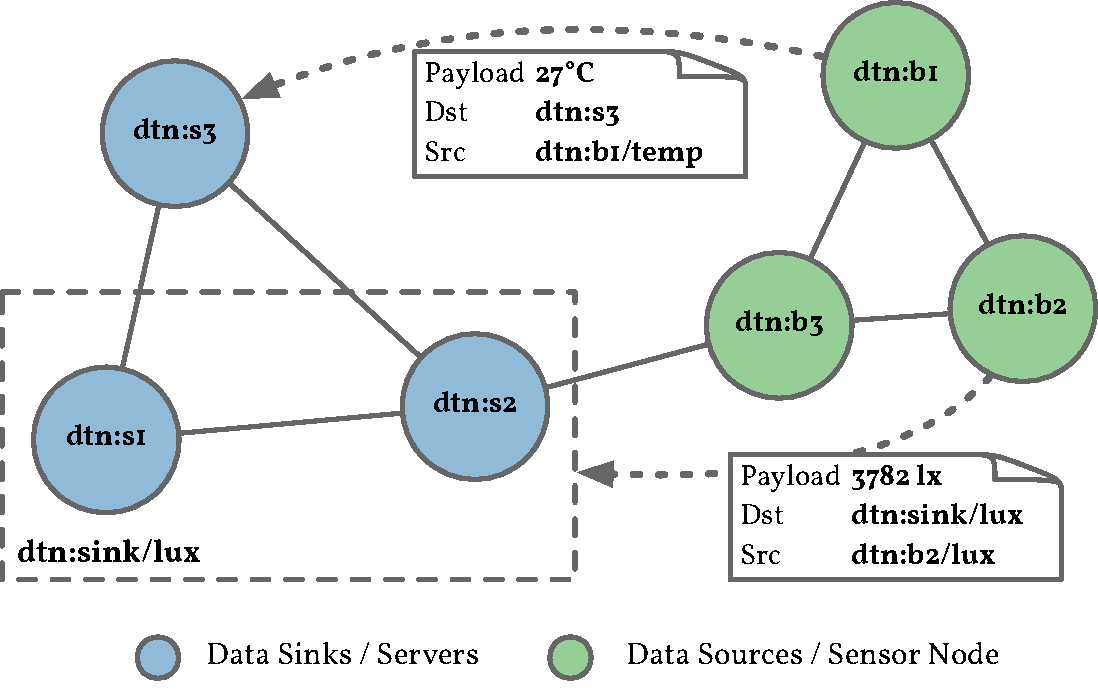
\includegraphics[width=0.6\linewidth,keepaspectratio]{include/nodes-endpoints}
  \end{figure}
\end{frame}
